\documentclass[11pt]{article}
\usepackage{graphicx}
\usepackage{float}
\usepackage{hyperref}
\usepackage{natbib}
\usepackage{listings}
\usepackage{xcolor}
\usepackage[dvipsnames]{xcolor}
\usepackage[svgnames]{xcolor}
\usepackage{amsmath} % For the equation* environment
\usepackage{amssymb}

\hypersetup{
    colorlinks=true,
    linkcolor=red,
    filecolor=cyan,      
    urlcolor=orange,
    pdftitle={Overleaf Example},
    pdfpagemode=FullScreen,
    }

\setlength{\textwidth}{6.5in}
\setlength{\headheight}{0in}
\setlength{\textheight}{8.0in}
\setlength{\hoffset}{0in}
\setlength{\voffset}{0in}
\setlength{\oddsidemargin}{0in}
\setlength{\evensidemargin}{0in}

\lstdefinestyle{txtstyle}{
    basicstyle=\ttfamily\small,
    breaklines=true,
    backgroundcolor=\color{Bisque}
}
\lstset{style = txtstyle}

\definecolor{codegreen}{rgb}{0,0.6,0}
\definecolor{codegray}{rgb}{0.5,0.5,0.5}
\definecolor{codepurple}{rgb}{0.58,0,0.82}
\definecolor{backcolour}{rgb}{0.95,0.95,0.92}

\lstdefinestyle{mystyle}{
    backgroundcolor=\color{backcolour},   
    commentstyle=\color{codegreen},
    keywordstyle=\color{magenta},
    numberstyle=\tiny\color{codegray},
    stringstyle=\color{codepurple},
    basicstyle=\ttfamily\footnotesize,
    breakatwhitespace=false,         
    breaklines=true,                 
    captionpos=b,                    
    keepspaces=true,                                   
    numbersep=5pt,                  
    showspaces=false,                
    showstringspaces=false,
    showtabs=false,                  
    tabsize=2
}

\title{Computational Physics ps-8 Report}
  
\author{Tongzhou Wang, \\ GitHub account: TZW56203, repository: phys-ga2000. \\ \url{https://github.com/TZW56203/phys-ga2000}}

\date{November 2, 2024}

\begin{document}

\maketitle

\section{Problem 1}
Listing \ref{lst:likemax} shows the maximum likelihood values, formal errors, and covariance matrix of $\beta_0$ and $\beta_1$.
\lstinputlisting[caption={Likelihood maximization.}, label={lst:likemax}]{code/ps-8-1.txt}

Figure \ref{fig:SandL} shows the survey results and the logistic model.
\begin{figure}[H]
    \centering
    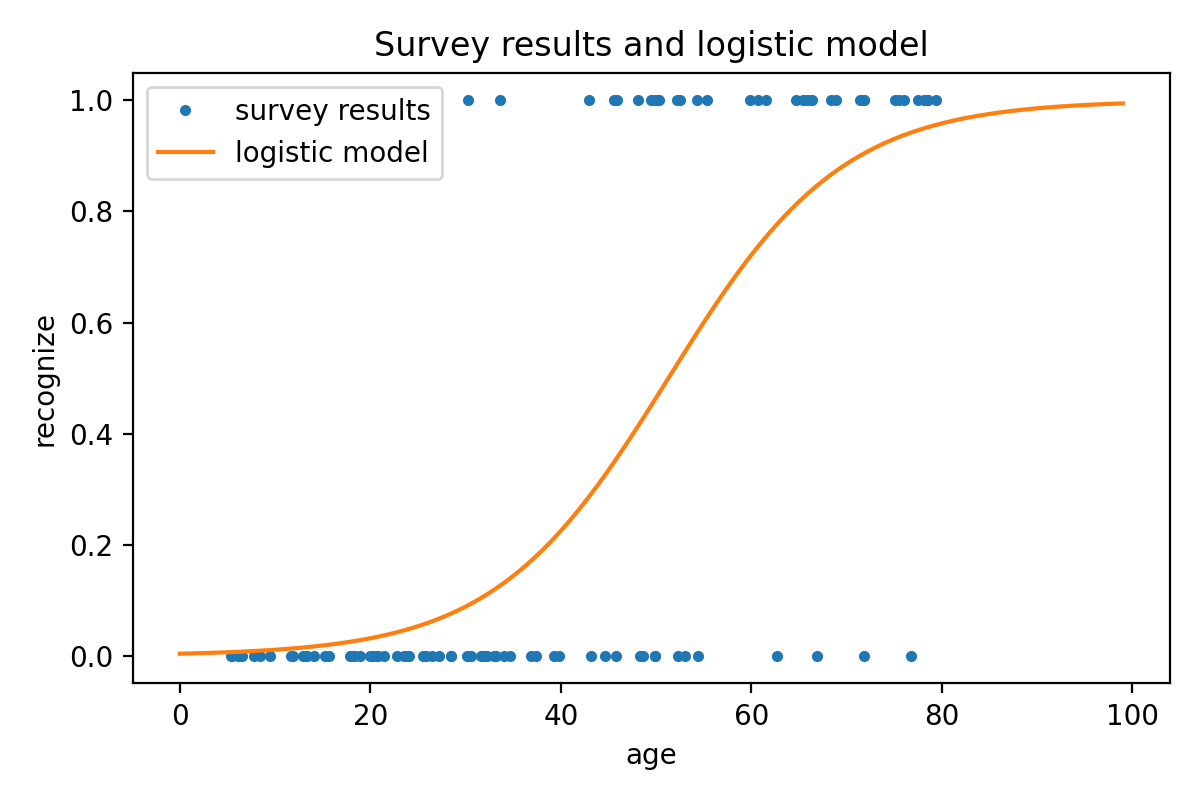
\includegraphics[scale = 0.8]{images/ps-8-1.png}
    \caption{Survey results and logistic model.}
    \label{fig:SandL}
\end{figure}

The logistic model seems to make sense because it gives a probability distribution that seems to explain the survey results, as shown in Figure \ref{fig:SandL}. For example, the logistic model is nearly zero between 0 and 20, and indeed no respondents between 0 and 20 years old recognizes the phrase.

\section{Problem 2}

\subsection{Part (a)}
The waveforms of the note played on a piano and a trumpet are shown in Figure \ref{fig:piano}, \ref{fig:trumpet}, and \ref{fig:pt}.
\begin{figure}[H]
    \centering
    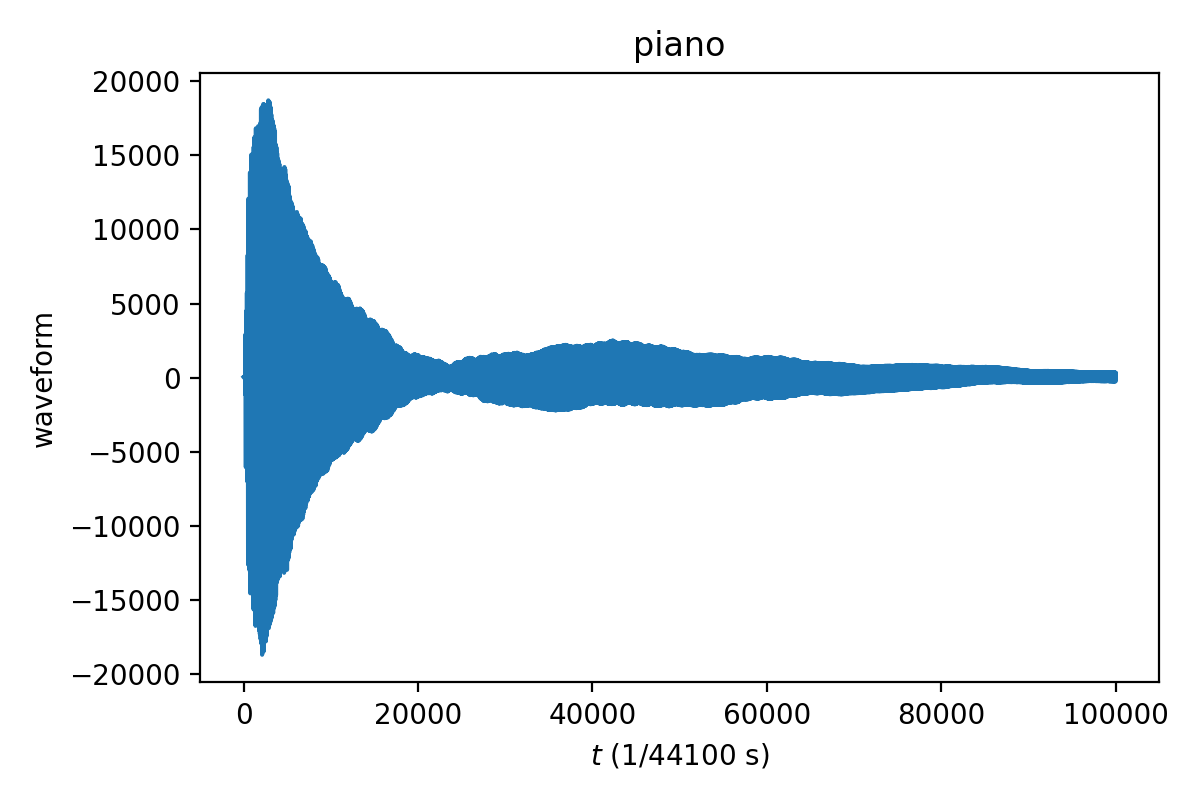
\includegraphics[scale = 0.6]{images/ps-8-2p.png}
    \caption{Piano.}
    \label{fig:piano}
\end{figure}
\begin{figure}[H]
    \centering
    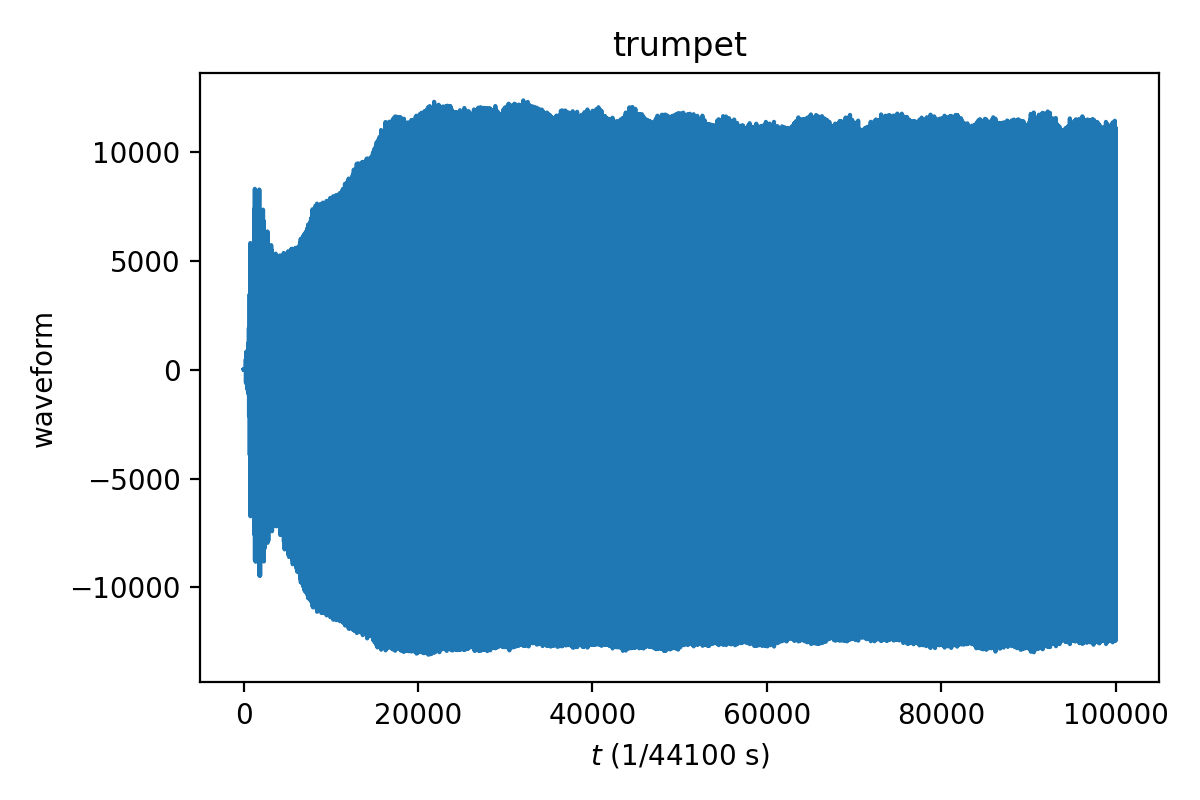
\includegraphics[scale = 0.6]{images/ps-8-2t.png}
    \caption{Trumpet.}
    \label{fig:trumpet}
\end{figure}
\begin{figure}[H]
    \centering
    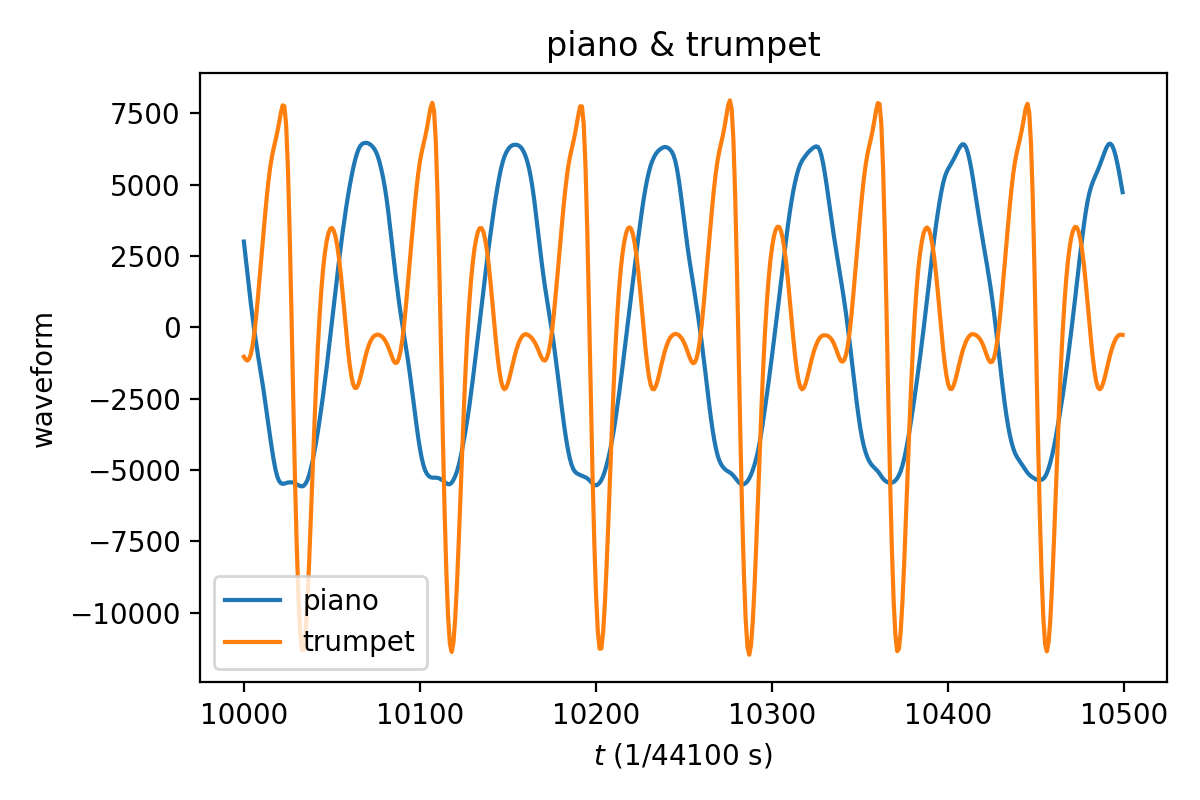
\includegraphics[scale = 0.8]{images/ps-8-2pt.png}
    \caption{Piano and trumpet.}
    \label{fig:pt}
\end{figure}

Figure \ref{fig:FTp} and \ref{fig:FTt} show magnitudes of the first 10000 Fourier coefficients of the discrete Fourier transforms. We can conclude that the sound of the piano is more precise because only the first harmonic has large Fourier coefficient. On the other hand, the sound of the trumpet contains several higher harmonics.

\begin{figure}[H]
    \centering
    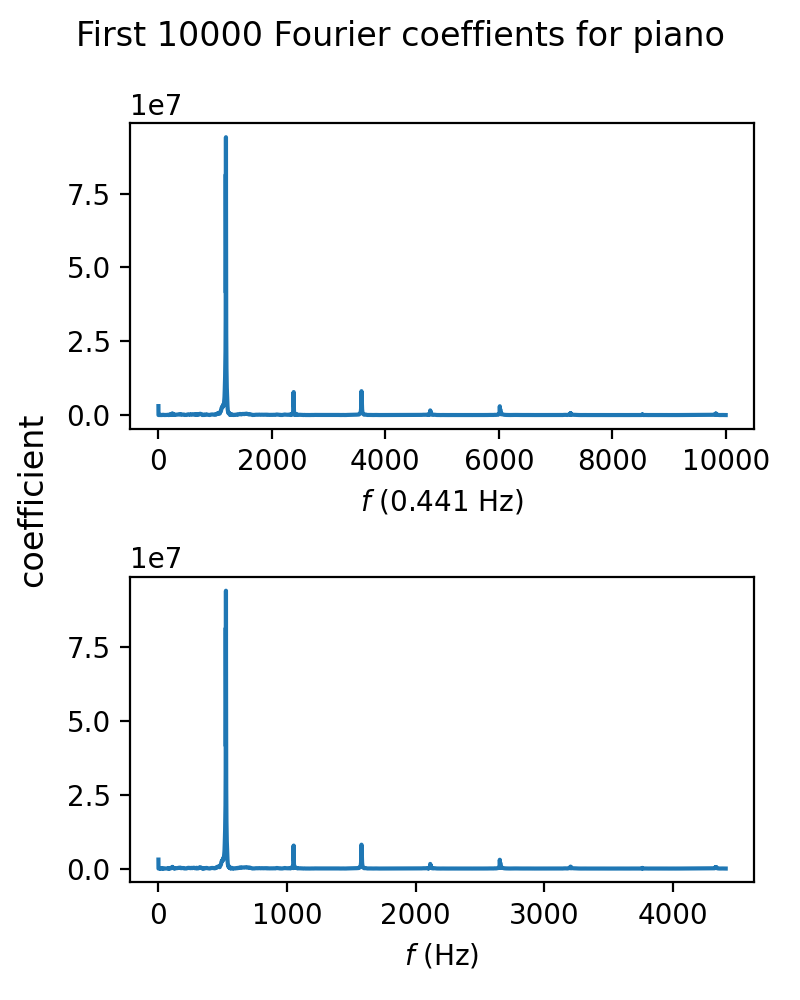
\includegraphics[scale = 0.68]{images/ps-8-2FTp.png}
    \caption{First 10000 Fourier coefficients for piano.}
    \label{fig:FTp}
\end{figure}
\begin{figure}[H]
    \centering
    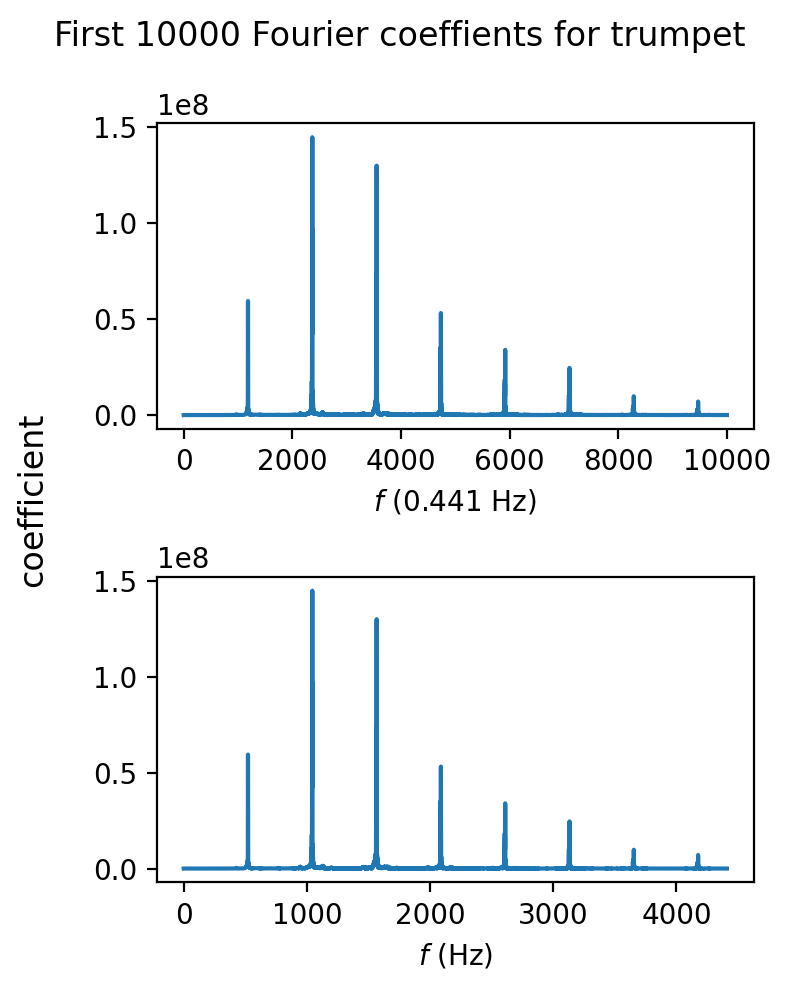
\includegraphics[scale = 0.68]{images/ps-8-2FTt.png}
    \caption{First 10000 Fourier coefficients for trumpet.}
    \label{fig:FTt}
\end{figure}

\subsection{Part (b)}
Listing \ref{lst:harmonics} shows the piano and trumpet frequencies where the Fourier coefficients are large. According to \url{https://en.wikipedia.org/wiki/Scientific_pitch_notation}, the frequency of $\mathrm{C}_5$ is 523.2511 Hz. We can conclude that the piano and the trumpet are playing $\mathrm{C}_5$.
\lstinputlisting[caption={Harmonics.}, label={lst:harmonics}]{code/ps-8-2.txt}

\section{Problem 3}
Figure \ref{fig:dow} shows the original data and the inverse Fourier transforms where all but the first 10\% and 2\% of the Fourier coefficients are set to zero. We can see that the general trend of the original plot is preserved, and the plot becomes smoother.
\begin{figure}[H]
    \centering
    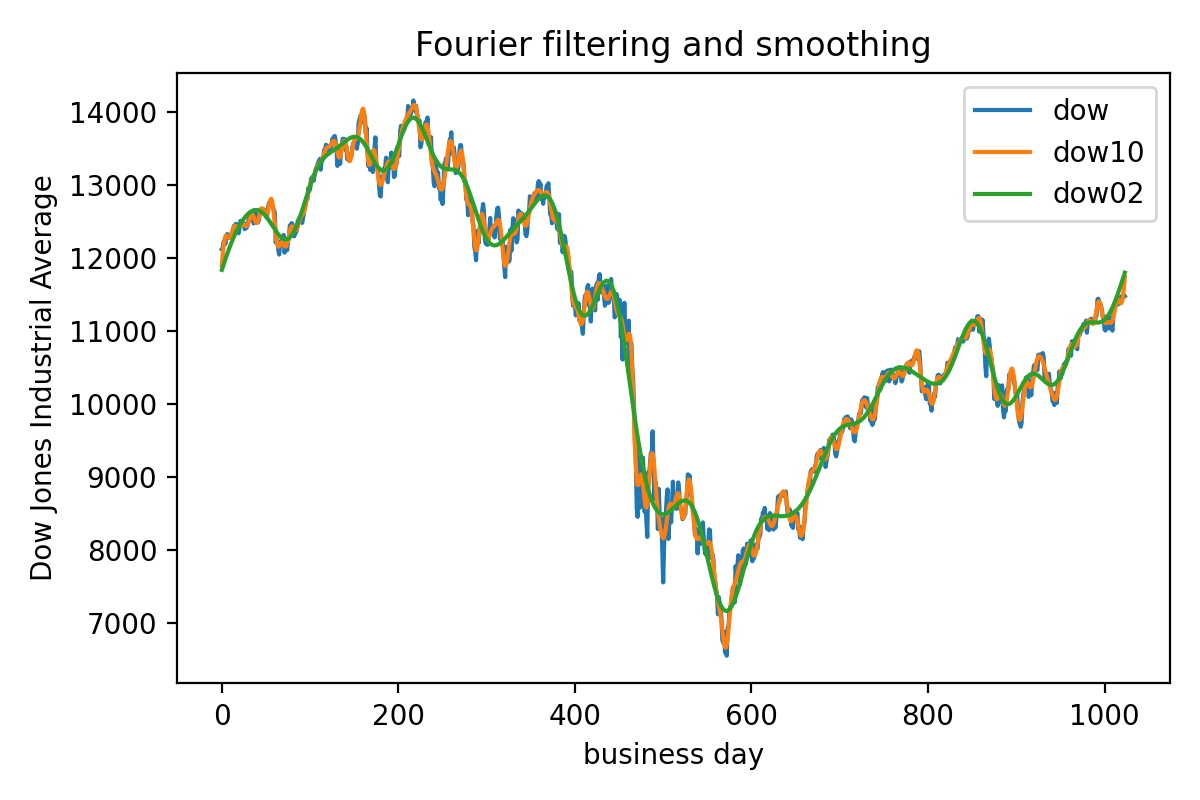
\includegraphics[scale = 0.8]{images/ps-8-3.png}
    \caption{Fourier filtering and smoothing.}
    \label{fig:dow}
\end{figure}

\end{document}
